\documentclass{standalone}
\usepackage{tikz}
\usetikzlibrary{patterns, positioning}


\begin{document}
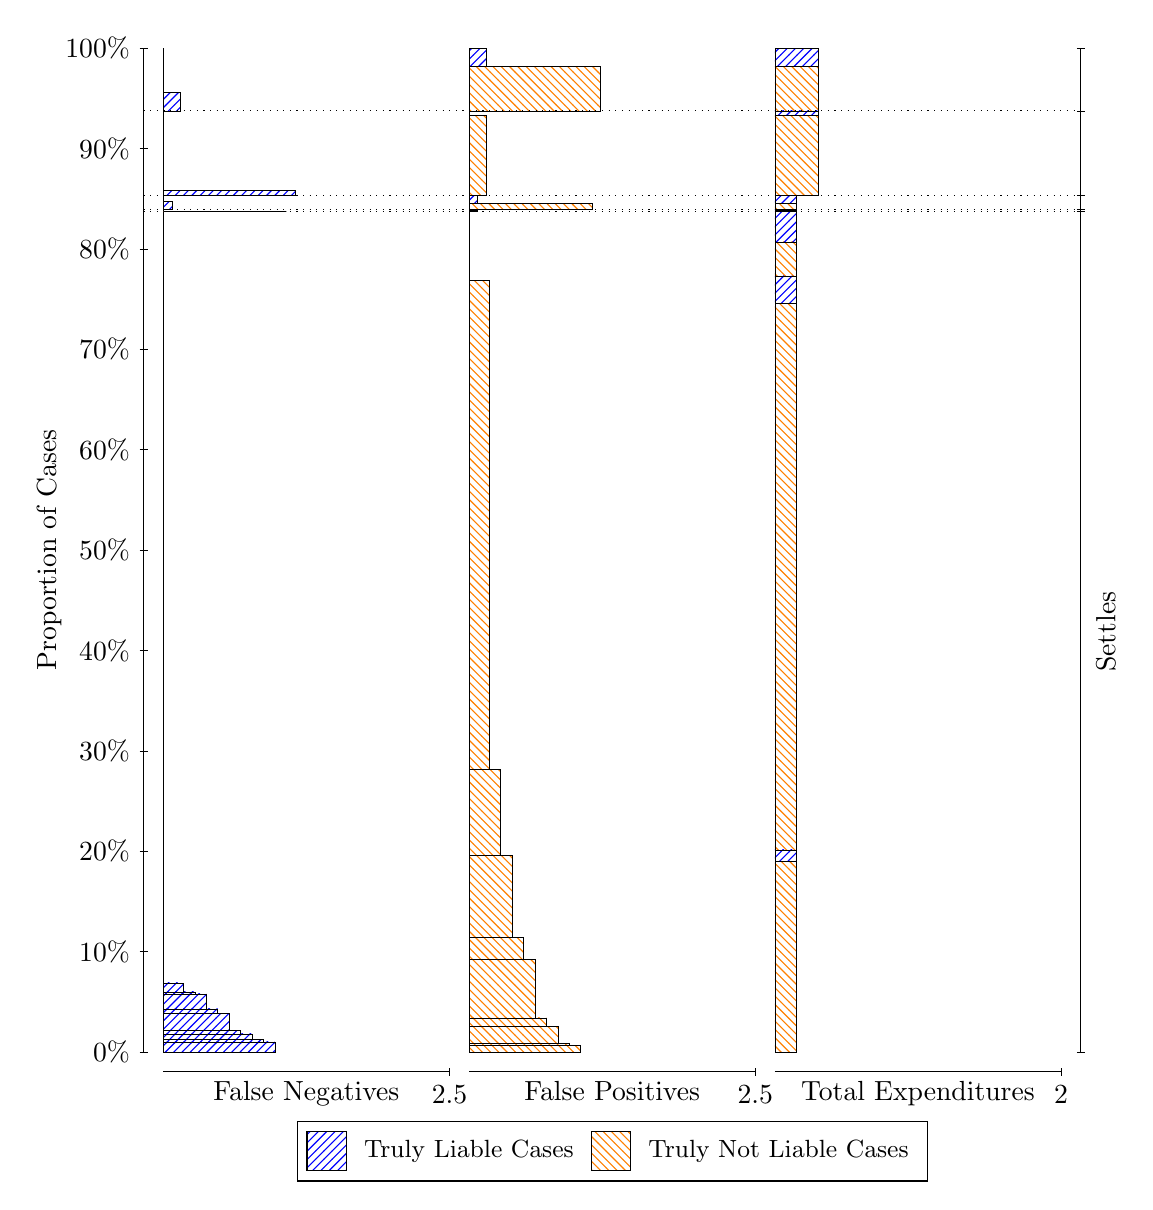
\begin{tikzpicture}
\draw[black, very thin] (1.5,1.75) -- (1.5,14.5);
\node[rotate=90, text=black, anchor=center] at (0.3, 8.125) {Proportion of Cases};
\draw[black, very thin] (1.45,1.75) -- (1.55,1.75);
\node[text=black, anchor=east] at (1.45, 1.75) {0\%};
\draw[black, very thin] (1.45,3.025) -- (1.55,3.025);
\node[text=black, anchor=east] at (1.45, 3.025) {10\%};
\draw[black, very thin] (1.45,4.3) -- (1.55,4.3);
\node[text=black, anchor=east] at (1.45, 4.3) {20\%};
\draw[black, very thin] (1.45,5.575) -- (1.55,5.575);
\node[text=black, anchor=east] at (1.45, 5.575) {30\%};
\draw[black, very thin] (1.45,6.85) -- (1.55,6.85);
\node[text=black, anchor=east] at (1.45, 6.85) {40\%};
\draw[black, very thin] (1.45,8.125) -- (1.55,8.125);
\node[text=black, anchor=east] at (1.45, 8.125) {50\%};
\draw[black, very thin] (1.45,9.4) -- (1.55,9.4);
\node[text=black, anchor=east] at (1.45, 9.4) {60\%};
\draw[black, very thin] (1.45,10.675) -- (1.55,10.675);
\node[text=black, anchor=east] at (1.45, 10.675) {70\%};
\draw[black, very thin] (1.45,11.95) -- (1.55,11.95);
\node[text=black, anchor=east] at (1.45, 11.95) {80\%};
\draw[black, very thin] (1.45,13.225) -- (1.55,13.225);
\node[text=black, anchor=east] at (1.45, 13.225) {90\%};
\draw[black, very thin] (1.45,14.5) -- (1.55,14.5);
\node[text=black, anchor=east] at (1.45, 14.5) {100\%};

\draw[black, very thin] (13.4,1.75) -- (13.4,14.5);
\draw[black, very thin] (13.35,1.75) -- (13.45,1.75);
\node[anchor=west] at (13.35, 1.75) {};
\draw[black, very thin] (13.35,12.426) -- (13.45,12.426);
\node[anchor=west] at (13.35, 12.426) {};
\draw[black, very thin] (13.35,12.446) -- (13.45,12.446);
\node[anchor=west] at (13.35, 12.446) {};
\draw[black, very thin] (13.35,12.63) -- (13.45,12.63);
\node[anchor=west] at (13.35, 12.63) {};
\draw[black, very thin] (13.35,13.703) -- (13.45,13.703);
\node[anchor=west] at (13.35, 13.703) {};
\draw[black, very thin] (13.35,14.5) -- (13.45,14.5);
\node[anchor=west] at (13.35, 14.5) {};

\draw[black, very thin, pattern color=blue, pattern=north east lines] (1.75,1.75) rectangle (3.167,1.8775);
\draw[black, very thin, pattern color=blue, pattern=north east lines] (1.75,1.8775) rectangle (3.0217,1.9076);
\draw[black, very thin, pattern color=blue, pattern=north east lines] (1.75,1.9076) rectangle (2.8763,1.9799);
\draw[black, very thin, pattern color=blue, pattern=north east lines] (1.75,1.9799) rectangle (2.731,2.0231);
\draw[black, very thin, pattern color=blue, pattern=north east lines] (1.75,2.0231) rectangle (2.5857,2.2404);
\draw[black, very thin, pattern color=blue, pattern=north east lines] (1.75,2.2404) rectangle (2.4403,2.2964);
\draw[black, very thin, pattern color=blue, pattern=north east lines] (1.75,2.2964) rectangle (2.295,2.4878);
\draw[black, very thin, pattern color=blue, pattern=north east lines] (1.75,2.4878) rectangle (2.1497,2.5143);
\draw[black, very thin, pattern color=blue, pattern=north east lines] (1.75,2.5143) rectangle (2.0043,2.6281);
\draw[black, very thin, pattern color=orange, pattern=north west lines] (1.75,2.6281) rectangle (1.75,12.426);
\draw[black, very thin, pattern color=blue, pattern=north east lines] (1.75,12.426) rectangle (3.3123,12.426);
\draw[black, very thin, pattern color=orange, pattern=north west lines] (1.75,12.426) rectangle (1.75,12.446);
\draw[black, very thin, pattern color=blue, pattern=north east lines] (1.75,12.446) rectangle (1.859,12.548);
\draw[black, very thin, pattern color=orange, pattern=north west lines] (1.75,12.548) rectangle (1.75,12.63);
\draw[black, very thin, pattern color=blue, pattern=north east lines] (1.75,12.63) rectangle (3.4213,12.692);
\draw[black, very thin, pattern color=orange, pattern=north west lines] (1.75,12.692) rectangle (1.75,13.703);
\draw[black, very thin, pattern color=blue, pattern=north east lines] (1.75,13.703) rectangle (1.968,13.935);
\draw[black, very thin, pattern color=orange, pattern=north west lines] (1.75,13.935) rectangle (1.75,14.5);
\draw[black, very thin, pattern color=orange, pattern=north west lines] (5.6333,1.75) rectangle (7.0503,1.8321);
\draw[black, very thin, pattern color=orange, pattern=north west lines] (5.6333,1.8321) rectangle (6.905,1.8579);
\draw[black, very thin, pattern color=orange, pattern=north west lines] (5.6333,1.8579) rectangle (6.7597,2.0734);
\draw[black, very thin, pattern color=orange, pattern=north west lines] (5.6333,2.0734) rectangle (6.6143,2.1831);
\draw[black, very thin, pattern color=orange, pattern=north west lines] (5.6333,2.1831) rectangle (6.469,2.9228);
\draw[black, very thin, pattern color=orange, pattern=north west lines] (5.6333,2.9228) rectangle (6.3237,3.2021);
\draw[black, very thin, pattern color=orange, pattern=north west lines] (5.6333,3.2021) rectangle (6.1783,4.2419);
\draw[black, very thin, pattern color=orange, pattern=north west lines] (5.6333,4.2419) rectangle (6.033,5.3429);
\draw[black, very thin, pattern color=orange, pattern=north west lines] (5.6333,5.3429) rectangle (5.8877,11.548);
\draw[black, very thin, pattern color=blue, pattern=north east lines] (5.6333,11.548) rectangle (5.6333,12.426);
\draw[black, very thin, pattern color=orange, pattern=north west lines] (5.6333,12.426) rectangle (5.7423,12.445);
\draw[black, very thin, pattern color=blue, pattern=north east lines] (5.6333,12.445) rectangle (5.6333,12.446);
\draw[black, very thin, pattern color=orange, pattern=north west lines] (5.6333,12.446) rectangle (7.1957,12.528);
\draw[black, very thin, pattern color=blue, pattern=north east lines] (5.6333,12.528) rectangle (5.7423,12.63);
\draw[black, very thin, pattern color=orange, pattern=north west lines] (5.6333,12.63) rectangle (5.8513,13.641);
\draw[black, very thin, pattern color=blue, pattern=north east lines] (5.6333,13.641) rectangle (5.6333,13.703);
\draw[black, very thin, pattern color=orange, pattern=north west lines] (5.6333,13.703) rectangle (7.3047,14.268);
\draw[black, very thin, pattern color=blue, pattern=north east lines] (5.6333,14.268) rectangle (5.8513,14.5);
\draw[black, very thin, pattern color=orange, pattern=north west lines] (9.5167,1.75) rectangle (9.7892,4.1701);
\draw[black, very thin, pattern color=blue, pattern=north east lines] (9.5167,4.1701) rectangle (9.7892,4.3157);
\draw[black, very thin, pattern color=orange, pattern=north west lines] (9.5167,4.3157) rectangle (9.7892,11.26);
\draw[black, very thin, pattern color=blue, pattern=north east lines] (9.5167,11.26) rectangle (9.7892,11.605);
\draw[black, very thin, pattern color=orange, pattern=north west lines] (9.5167,11.605) rectangle (9.7892,12.038);
\draw[black, very thin, pattern color=blue, pattern=north east lines] (9.5167,12.038) rectangle (9.7892,12.426);
\draw[black, very thin, pattern color=orange, pattern=north west lines] (9.5167,12.426) rectangle (9.7892,12.445);
\draw[black, very thin, pattern color=blue, pattern=north east lines] (9.5167,12.445) rectangle (9.7892,12.446);
\draw[black, very thin, pattern color=orange, pattern=north west lines] (9.5167,12.446) rectangle (9.7892,12.528);
\draw[black, very thin, pattern color=blue, pattern=north east lines] (9.5167,12.528) rectangle (9.7892,12.63);
\draw[black, very thin, pattern color=orange, pattern=north west lines] (9.5167,12.63) rectangle (10.062,13.641);
\draw[black, very thin, pattern color=blue, pattern=north east lines] (9.5167,13.641) rectangle (10.062,13.703);
\draw[black, very thin, pattern color=orange, pattern=north west lines] (9.5167,13.703) rectangle (10.062,14.268);
\draw[black, very thin, pattern color=blue, pattern=north east lines] (9.5167,14.268) rectangle (10.062,14.5);
\draw[black, dotted] (1.5,12.426) -- (13.4,12.426);
\draw[black, dotted] (1.5,12.446) -- (13.4,12.446);
\draw[black, dotted] (1.5,12.63) -- (13.4,12.63);
\draw[black, dotted] (1.5,13.703) -- (13.4,13.703);
\draw[black, very thin] (1.75,1.5) -- (5.3833,1.5);
\node[text=black, anchor=north] at (3.5667, 1.5) {False Negatives};
\draw[black, very thin] (5.3833,1.45) -- (5.3833,1.55);
\node[text=black, anchor=north] at (5.3833, 1.45) {2.5};

\draw[black, very thin] (5.6333,1.5) -- (9.2667,1.5);
\node[text=black, anchor=north] at (7.45, 1.5) {False Positives};
\draw[black, very thin] (9.2667,1.45) -- (9.2667,1.55);
\node[text=black, anchor=north] at (9.2667, 1.45) {2.5};

\draw[black, very thin] (9.5167,1.5) -- (13.15,1.5);
\node[text=black, anchor=north] at (11.333, 1.5) {Total Expenditures};
\draw[black, very thin] (13.15,1.45) -- (13.15,1.55);
\node[text=black, anchor=north] at (13.15, 1.45) {2};

\node[text=black, centered, rotate=90] at (13.72, 7.0879) {Settles};





\draw (7.449999999999999,1.5) node[draw=none] (baseCoordinate) {};
\begin{scope}[align=center]
        \matrix[scale=0.5, draw=black, below=0.5cm of baseCoordinate, nodes={draw}, column sep=0.1cm]{
            \node[rectangle, draw, minimum width=0.5cm, minimum height=0.5cm, pattern color=blue, pattern=north east lines] {}; &
            \node[draw=none, font=\small, text=black] (B) {Truly Liable Cases}; &
            \node[rectangle, draw, minimum width=0.5cm, minimum height=0.5cm, pattern color=orange, pattern=north west lines] {}; &
            \node[draw=none, font=\small, text=black] (B) {Truly Not Liable Cases}; \\
            };
\end{scope}

\end{tikzpicture}
\end{document}